\documentclass[border=6pt]{standalone}
\usepackage{tikz}
\usepackage[edges]{forest}
\usetikzlibrary{arrows.meta,positioning,calc,decorations.pathreplacing,shapes.geometric}
\begin{document}
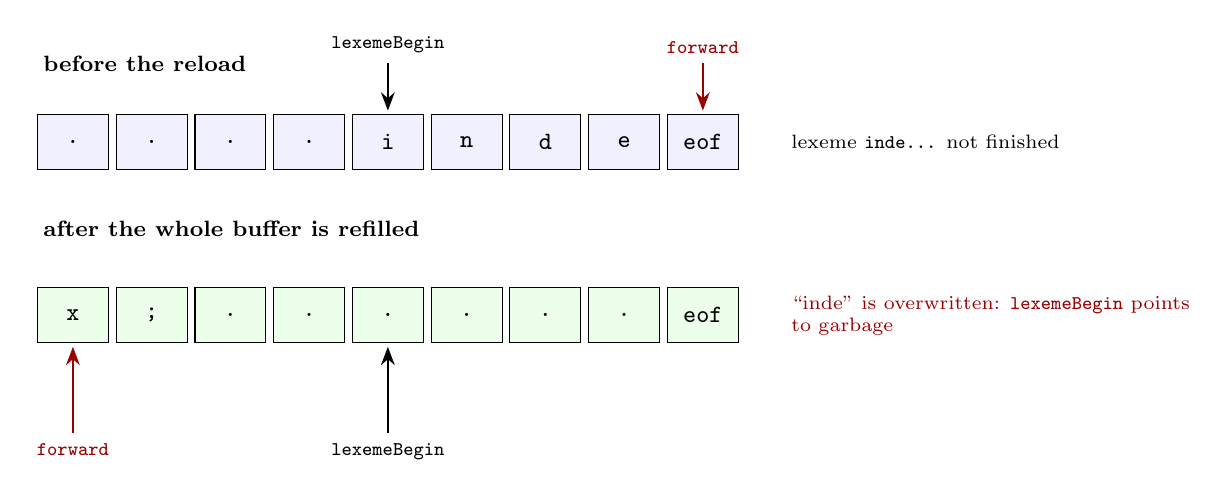
\begin{tikzpicture}[>=Stealth,font=\small,
 cell/.style={draw,minimum width=0.9cm,minimum height=0.7cm,font=\ttfamily\small}]
\node[font=\footnotesize\bfseries,anchor=west] at (-0.5,2.0) {before the reload};
\foreach \i/\c in {0/.,1/.,2/.,3/.,4/i,5/n,6/d,7/e,8/eof} \node[cell,fill=blue!6] at (\i,1.0) {\c};
\draw[->,thick] (4,2.0) node[above,font=\scriptsize\ttfamily]{lexemeBegin} -- (4,1.4);
\draw[->,thick,red!60!black] (8,2.0) node[above,font=\scriptsize\ttfamily]{forward} -- (8,1.4);
\node[font=\scriptsize,anchor=west] at (9.0,1.0) {lexeme \texttt{inde...} not finished};
\node[font=\footnotesize\bfseries,anchor=west] at (-0.5,-0.1) {after the whole buffer is refilled};
\foreach \i/\c in {0/x,1/;,2/.,3/.,4/.,5/.,6/.,7/.,8/eof} \node[cell,fill=green!8] at (\i,-1.2) {\c};
\draw[->,thick,red!60!black] (0,-2.7) node[below,font=\scriptsize\ttfamily]{forward} -- (0,-1.6);
\draw[->,thick] (4,-2.7) node[below,font=\scriptsize\ttfamily]{lexemeBegin} -- (4,-1.6);
\node[font=\scriptsize,anchor=west,red!60!black,align=left] at (9.0,-1.2) {``inde'' is overwritten: \texttt{lexemeBegin}\ points\\to garbage};
\end{tikzpicture}
\end{document}
